\begin{figure}[H]
    \centering
    \begin{minipage}{0.45\textwidth}
        \centering
        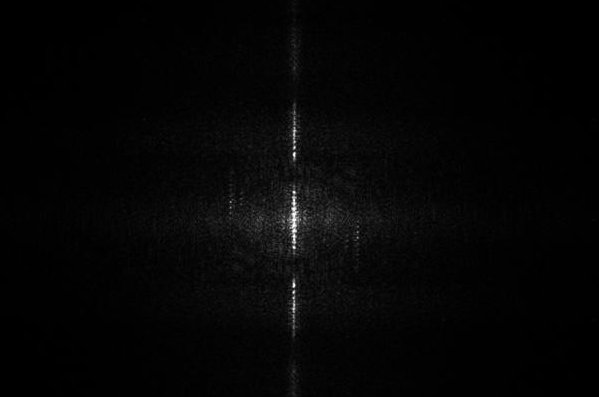
\includegraphics[ width = 0.95 \linewidth ]{figures/CalculatedFT/1505_FourierTransform_LinearPlot3.jpg}
        \caption{The calculated FT using filter 1}
    \end{minipage}%
    \begin{minipage}{0.45\textwidth}
        \centering
        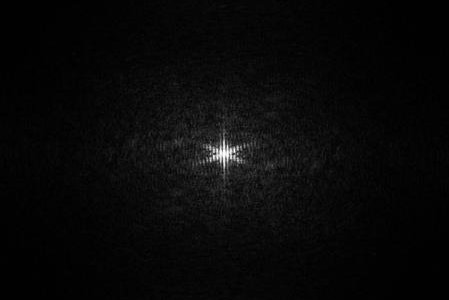
\includegraphics[ width = 0.95 \linewidth ]{figures/CalculatedFT/1508_FourierTransform_LinearPlot3.jpg}
        \caption{The calculated FT using filter 2}
    \end{minipage}%
    \vspace{2cm}
    \begin{minipage}{0.45\textwidth}
        \centering
        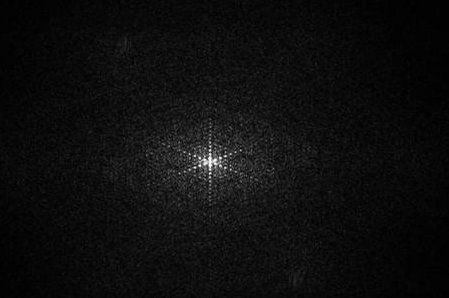
\includegraphics[ width = 0.95 \linewidth ]{figures/CalculatedFT/1511_FourierTransform_LinearPlot3.jpg}
        \caption{The calculated FT using filter 3}
    \end{minipage}%
    \begin{minipage}{0.45\textwidth}
        \centering
        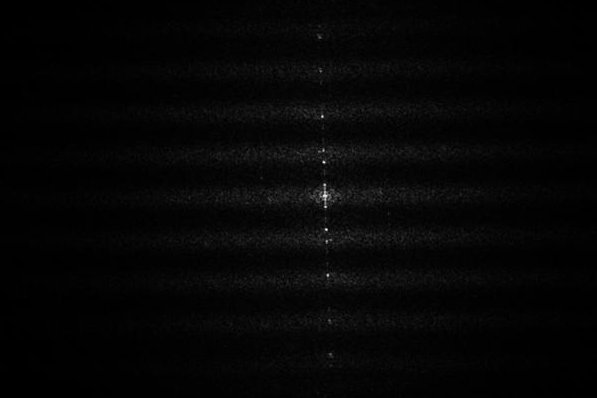
\includegraphics[ width = 0.95 \linewidth ]{figures/CalculatedFT/1514_FourierTransform_LinearPlot3.jpg}
        \caption{The calculated FT using filter 4}
    \end{minipage}%
    \vspace{2cm}
    \begin{minipage}{0.45\textwidth}
        \centering
        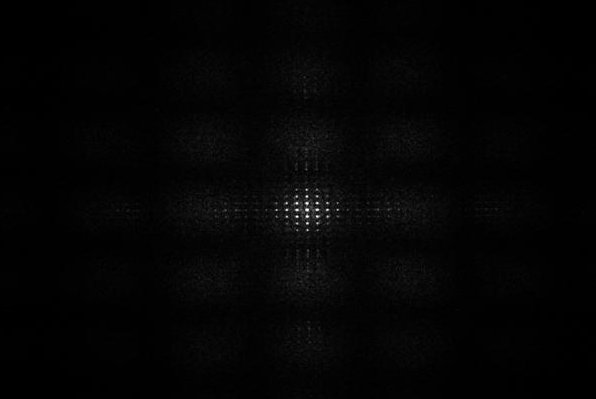
\includegraphics[ width = 0.95 \linewidth ]{figures/CalculatedFT/1517_FourierTransform_LinearPlot3.jpg}
        \caption{The calculated FT using filter 5}
    \end{minipage}%
    \begin{minipage}{0.45\textwidth}
        \centering
        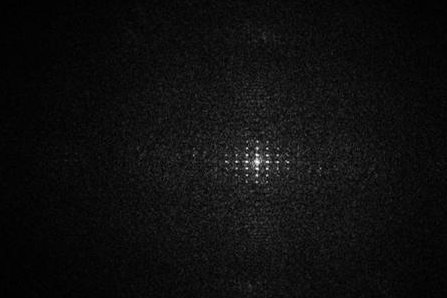
\includegraphics[ width = 0.95 \linewidth ]{figures/CalculatedFT/1520_FourierTransform_LinearPlot3.jpg}
        \caption{The calculated FT using filter 6}
    \end{minipage}%
\end{figure}